\documentclass[a4paper]{article}
\usepackage{amsmath}
\usepackage{graphicx}
\usepackage[utf8]{inputenc}
\usepackage[T1]{fontenc}
\usepackage[french]{babel}
\usepackage{amsfonts,amsmath,amssymb}
\usepackage{float}
\usepackage{graphicx}

\title{\textbf{Rapport d'alternance Master 2 Ingénierie logicielle\\ }}
\author{\textbf{MOUTARAJJI} Mouhyi-Eddine\
\\Encadré par :\\\textbf{SALAÜN} Gaël \\\textbf{BOURDÉ} Annabel }
\begin{document}
\date{}




\maketitle

\newpage

\tableofcontents
~
\newpage



\section{Rectorat de l’académie de Rennes} 

\subsection{Présentation}

Le rectorat de l'académie de Rennes est une circonscription administrative propre à
l’Éducation Nationale.\\
Elle regroupe 4 directions des services départementaux de l'Éducation Nationale : 
Côtes d'Armor, Finistère, Ille-et-Vilaine et Morbihan. Chaque direction des services départementaux de l'éducation nationale est placée sous la responsabilité d'un inspecteur d'académie, directeur académique des services de l'Éducation nationale.\\\\
Son rôle au sein de ces départements est de gérer les personnels, les élèves, les moyens financiers, les examens... de tous les établissements scolaires, depuis la maternelle jusqu'au lycée.\\\\

\subsection{L'architecture des projets}

Au sein du rectorat, les développeurs travaillent sur plusieurs types d'application (métier, outils ...). Ces applications sont constituées de deux modules: 

Un module Back-end : Le Back-End, c’est la partie du code qui est exécutée par le serveur, il s’agît d'un serveur fournissant une API gérant la persistance des données et la logique de l'application.La majorité des applications du rectorat sont développées en framwork Spring-boot et en langage Java et il existe quelques applications développées en langage Kotlin dont l'application Apptour.


Le back-end des applications se décomposent de plusieurs couches: 


une couche Repository/DAO: Repositories sont des interfaces héritant de l'interface Repository. L'objectif de ces interfaces consiste à rendre la création de la couche d'accès aux données (requêtes SELECT, UPDATE...) plus rapide.

une couche Service: Elle permet de séparer les opérations effectuées par le contrôleur et celles qui concernent le modèle des données. Toute action devrait passer par cette couche.

Une couche Contrôller: Il s'agit de l'Api qui permet de répondre à toutes les requêtes envoyées par le client. 

\begin{center}
 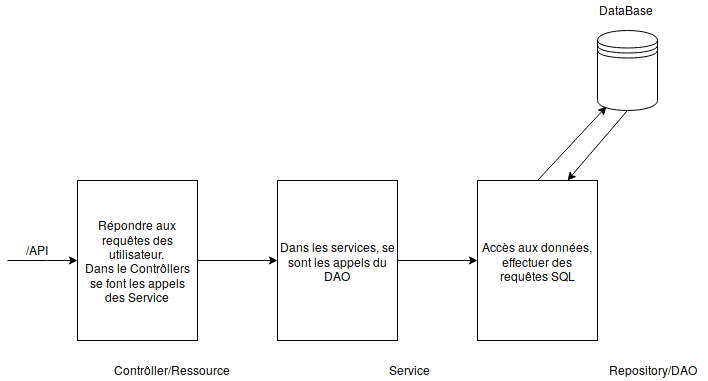
\includegraphics[width=1\textwidth]{diagrammes/ArchitectureProjet.png} 
\end{center}
Un module Front-end :

\end{document}
